
\section{Combination}


%This note presents a combined measurement of the \ttbar\ production cross-section at a center-of-mass energy of $\sqrt{s}= 7\, \TeV$ using ATLAS results in the single-lepton, dilepton, and all-hadronic channels.

The previous sections described individual analysis efforts used to measure the top-quark pair-production cross-section.
In this section, each of these measurements is combined to obtain a single measurement of the $\ttbar$ cross-section 
that uses the events of all three channels simultaneously.
This is performed by constructing likelihood functions for the three individual measurements, including the effect of all
systematic uncertainties, and using these to create a join likelihood that spans each individual analysis.
This combination results in a reduction in both statistical and systematic uncertainties.
The measurements being used in this simultaneous likelihood are the single-lepton~\cite{LEPTON_JETS_NOTE_2011} and dilepton~\cite{DILEPTON_PAPER} channels,
which used 0.70 \ifb\ of data, and the measurement in the all-hadronic channel, 
which used1.02 \ifb\ of data~\cite{ATLAS-CONF-2011-140}, all of which was taken in 2011 with the ATLAS detector.

%% The uncertainty on the integrated luminosity is estimated to be 3.7\%~\cite{luminew}.
%% The single-lepton channel measurements are based on a multivariate discriminant distribution that is simultaneously fit to both lepton final states, which are each divided into samples containing $3,4,$ and $\ge 5$ jets (Section~\ref{sec:lepjets}).
%% The measurements in the dilepton channel, which is comprised of electron-electron, electron-muon, and muon-muon final states, are cut-based analyses which require at least 2 jets (Section~\ref{sec:dilep}).
%% Dilepton measurements requiring only a single isolated lepton plus an isolated track or an isolated lepton plus a hadronically decaying $\tau$ are not used in this combination because they have significant overlap with events used in the single-lepton measurement~\cite{mutauCONF}.
%% % The measurements in the dilepton channel use || The dilepton channel is comp
%% For both the dilepton and single-lepton channels, no requirement on $b$-tagging is imposed.
%% The all-hadronic channel measurement is based on a binned maximum-likelihood fit of signal and background templates, which use the $\chi^2$ of the reconstructed top-quark mass per
%% event as a discriminant (Section~\ref{sec:allhad}).
%% %  where the discriminating variable for each event is the chi-square of a kinematic fit assuming the $\ttbar$ event hypothesis.
%% % of a chi-square of the reconstructed top-quark mass per event as a   discriminant
%% The results of the various cross-section measurements in the single-lepton, dilepton, and all-hadronic channels are shown in Table~\ref{tab:results}.
%% % Even though the dilepton and single-lepton analyses do not require $b$-tagging, the combination with the single-lepton channel assumes that the branching ratio of $t\to W b$ is $100\%$.

The likelihood for each of the channels is a function of the signal cross-section, $\sigma_{\ttbar}$, the integrated luminosity, $\lum$, and several nuisance parameters $\alpha_j$ that correspond to various sources of systematic uncertainty.
In the joint likelihood, a single parameter is used across all three analysis to represent the value of the $\ttbar$ cross-section.
In addition, the individual measurements share several common sources of systematic uncertainty,
which must be treated consistently in order to form a statistical combination (Section~\ref{sec:comb})
Therefore, when forming the six-measurement combined likelihood, constraint terms for systematic uncertainties that are common across analyses are included only once.

%that parametrize the effect of various sources of systematic uncertainty.
%The full combination is implemented as a product of the individual likelihoods of the component analyses. %, using approximations when necessary.
%The single-lepton likelihood function was approximated by a multivariate Gaussian with covariance given by the Hessian matrix from MINUIT's HESSE algorithm~\cite{minuit}.  

The final measurement of the $\ttbar$ cross-section is performed using the profile likelihood ratio,
which is designed to take into account the effect of nuisance parameters when evaluating the uncertainty on the measured cross-section:
\begin{equation}\label{Eq:lr_2}
  \lambda(\sigma_{\ttbar}) = \frac{L(\sigma_{\ttbar}, \hat{\hat{\lum}}, \hat{\hat{\alpha}}_j)}{L(\hat \sigma_{\ttbar}, \hat \lum, \hat \alpha_j)}\,,
\end{equation}
where  $\hat\sigma_{\ttbar}, \hat \lum, \hat\alpha_j$ denote the maximum likelihood estimate of all the parameters and  $\hat{\hat{\lum}}$ and $\hat{\hat{\alpha}}_j$ represent the conditional maximum likelihood estimates of $\lum$ and $\alpha_j$ holding $\sigma_{\ttbar}$ fixed.   
The best fit value of the cross-section is $\hat\sigma_{\ttbar}$ and the 68\% confidence interval is derived from the values of $\sigma_{\ttbar}$ which give $-2\log \lambda(\sigma_{\ttbar})= 1$~\cite{James:1994vp}~\cite{asimov}.


\subsection{Likelihood function for the Lepton + Jets Analysis}

\label{sec:lepjets}

%The likelihood function for the single-lepton channel is formed  the $e$+jets and $\mu$+jets models, taking into account common systematic uncertainties.  
The single-lepton channel, which consists of $e$+jets and $\mu$+jets final states, is described by a single likelihood function.
This likelihood function consists of the parameter of interest, $\sigma_{\ttbar}$, and 45 nuisance parameters $\vec{\alpha}$, 
which are together denoted $\vec{\theta} = (\sigma_{\ttbar}, \vec{\alpha})$.
The maximum likelihood estimator of this single-lepton combination is denoted $\hat{\vec{\theta}}$.
The largest sources of systematic uncertainty in the single-lepton channel come from the Monte Carlo generator for signal, the jet energy scale, and the modeling of initial-state and final-state radiation.
Uncertainties that affect the background only, including uncertainties on the shape of $W+$jets and QCD templates, contribute less than those affecting signal only.
More information on the cross-section measurement using single-lepton final states can be found in reference~\cite{LEPTON_JETS_NOTE_2011}.

For the purposes of the six-measurement combination, the likelihood from the single-lepton channels is approximated using a multivariate Gaussian.
This approximation facilitates the combination with the dilepton and all-hadronic likelihoods, which are implemented in a different software framework.  
Figure~\ref{fig:ljets_combined} shows $-\log\lambda(\sigma_{\ttbar})$ vs. $\sigma_{\ttbar}/\sigma_{\rm SM}$ for the single-lepton model using both the exact and the approximate likelihood.
It can be seen that the likelihood is very symmetric and parabolic, indicating that a multivariate Gaussian is a good approximation to the likelihood function. 
The covariance matrix used to construct the multivariate Gaussian comes from the Hessian matrix of the negative log-likelihood function evaluated at the best fit point:

% The largest contribution to the systematic uncertainty on the begin  comes from the choice of the signal MC generator followed by the uncertainties on the jet energy scale calibration and the modeling of initial and final state radiation.

% The uncertainties on the background modeling come from the uncertainty on the shape of W+jets and QCD templates


%  \begin{equation}
%  V_{ij}^{-1} = - \frac{\partial^2 }{\partial \theta_i \partial \theta_j} \log L(\vec{\theta})\; \bigg | \; {\hat{\vec{\theta}}} \; .
%  \end{equation}
%\end{minipage}
%\hspace{0.5cm}
%\begin{minipage}{0.7\linewidth}
%  \begin{equation}
%  L_{l+\rm jets}(\vec{\theta}) = G(\hat{\vec{\theta}}\, |\, \vec{\theta}, V) = \frac{1}{(2\pi)^{k/2} | V|^{1/2}} \exp\left( -\frac{1}{2} (\hat{\vec{\theta}} - \vec{\theta})^T  V^{-1} (\hat{\vec{\theta}} - \vec{\theta})  \right) \;, 
%  \end{equation}
%  \end{minipage}


\begin{equation}
  V_{ij}^{-1} = - \frac{\partial^2 }{\partial \theta_i \partial \theta_j} \log L(\vec{\theta})\; {\bigg | \;}_{\hat{\vec{\theta}}} \; \quad .
\end{equation}
With the covariance matrix, one can construct the multivariate Gaussian likelihood 
\begin{equation} \label{eqn:ljetsLikelihood}
  L_{l+\rm jets}(\vec{\theta}) = G(\hat{\vec{\theta}}\, |\, \vec{\theta}, V) = \frac{1}{(2\pi)^{k/2} | V|^{1/2}} \exp\left( -\frac{1}{2} (\hat{\vec{\theta}} - \vec{\theta})^T  V^{-1} (\hat{\vec{\theta}} - \vec{\theta})  \right) \;, 
\end{equation}
where $k=46$ is the dimensionality of the parameter space.  
Uncertainties that are evaluated outside of the fit in in reference~\cite{LEPTON_JETS_NOTE_2011} are here modeled as factors which scale $\sigma_{\ttbar}/\sigma_{\rm SM}$ and are described by Gaussian terms.
%Uncertainties that are evaluated outside of the fit in the single-lepton analysis are here modeled as scalings on $\sigma_{\ttbar}/\sigma_{\rm SM}$ and are constrained by Gaussian terms.
%Uncertainties that are evaluated outside of the fit in the single-lepton analysis are here modeled as parameterized uncertainties on $\sigma_{\ttbar}/\sigma_{\rm SM}$ in the multivariate gaussian likelihood.


\begin{figure}[htbp]
  \begin{center}
    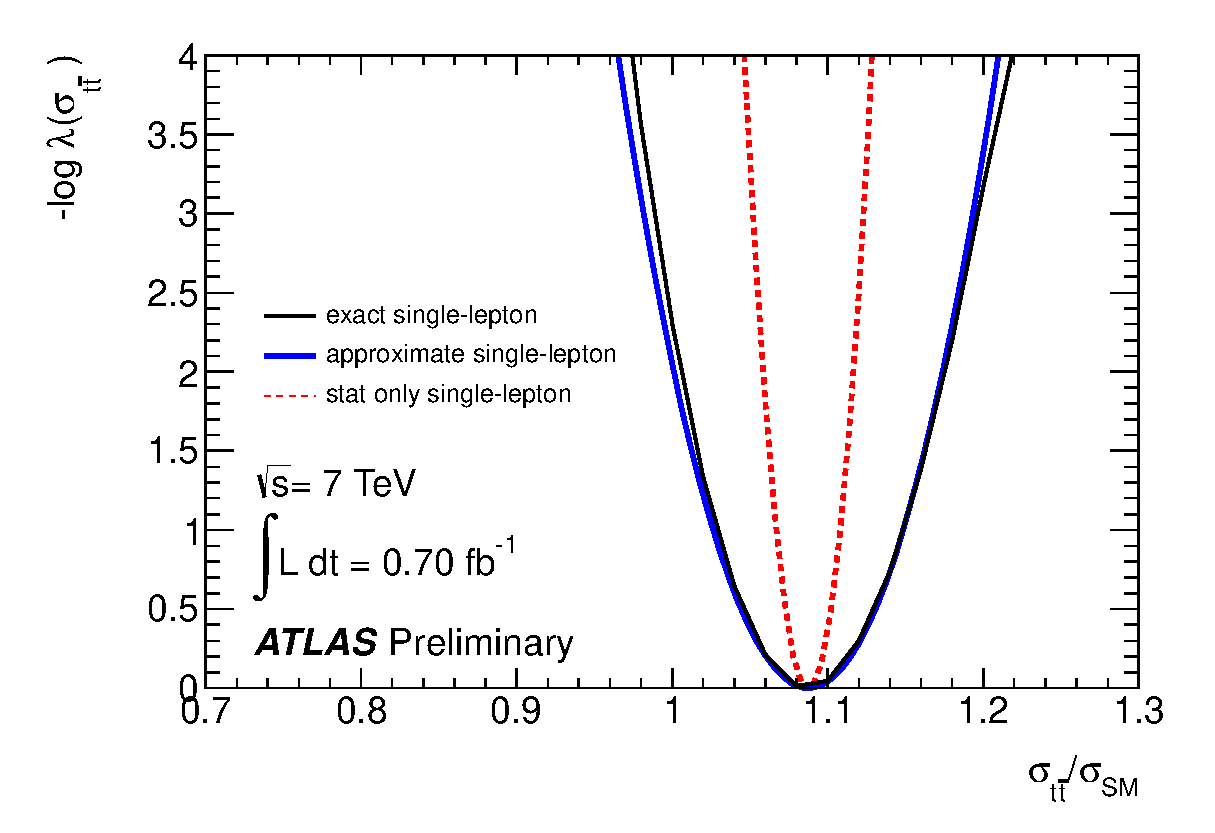
\includegraphics[width=.5\textwidth]{figures/comb/ljets_likelihood_curve}
    \caption{Graph of $-\log\lambda(\sigma_{\ttbar})$ vs. $\sigma_{\ttbar}/\sigma_{\rm SM}$ for both the exact (black, solid) and approximate (blue, solid) $l$+jets likelihood~\cite{LEPTON_JETS_NOTE_2011}.  
The same graph using the approximate likelihood without systematic uncertainties (red, dashed) is also shown.  
The likelihoods shown here do not include systematics that are evaluated outside of the fit.}
    %\includegraphics[width=.5\textwidth]{figures/comb/ljets_likelihood_curve_ljets_onePlot.eps}
    %\caption{Graph of $-\log\lambda(\sigma_{\ttbar})$ vs. $\sigma_{\ttbar}/\sigma_{\rm SM}$ for the $l$+jets combined likelihood.}
    \label{fig:ljets_combined}
  \end{center}
\end{figure}

%\begin{figure}[htbp]
%  \begin{center}
%    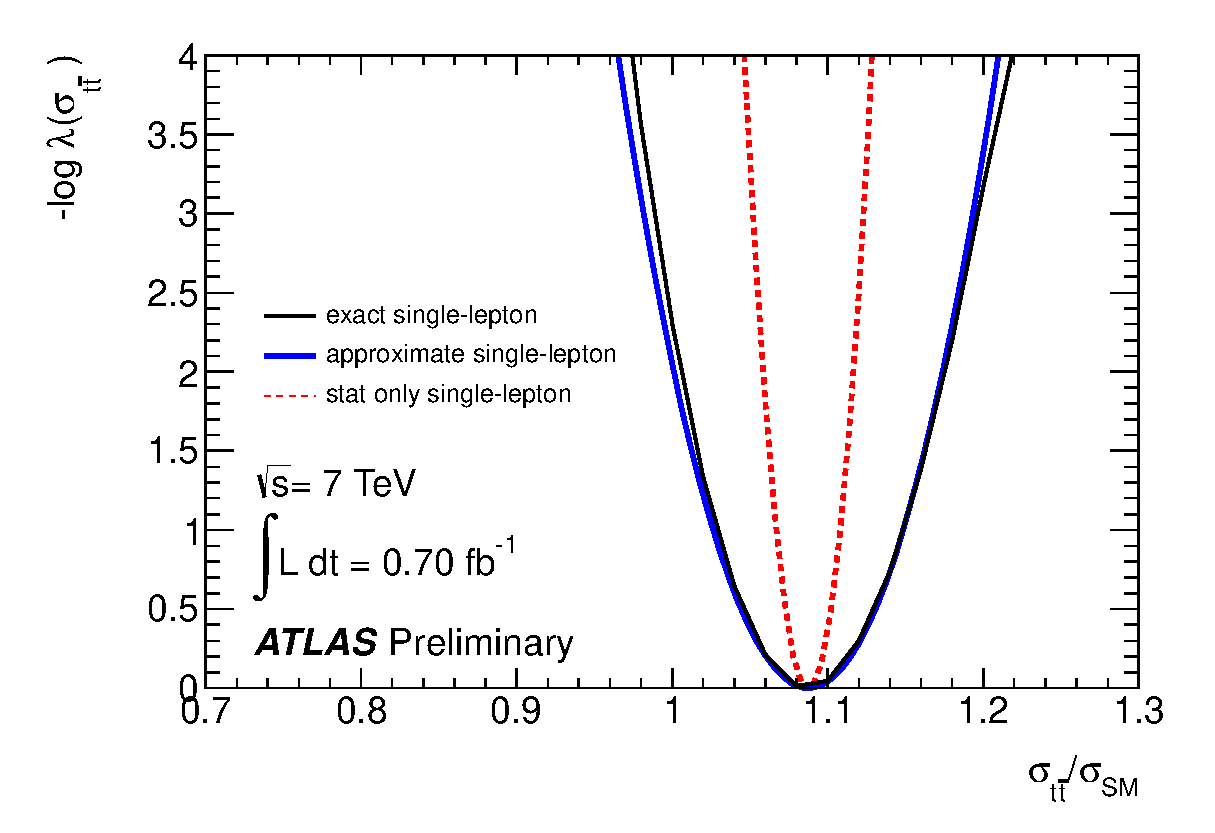
\includegraphics[width=.5\textwidth]{figures/comb/ljets_likelihood_curve.eps}
%    \caption{Graphs of $-\log\lambda(\sigma_{\ttbar})$ vs. $\sigma_{\ttbar}/\sigma_{\rm SM}$ from the $e$+jets (green, dashed), $\mu$+jets (blue, dashed), and $l$+jets combined likelihood (black, solid).  The likelihoods do not include systematics that are evaluated outside of the fit.}
%    %\includegraphics[width=.5\textwidth]{figures/comb/ljets_likelihood_curve_ljets_onePlot.eps}
%    %\caption{Graph of $-\log\lambda(\sigma_{\ttbar})$ vs. $\sigma_{\ttbar}/\sigma_{\rm SM}$ for the $l$+jets combined likelihood.}
%    \label{fig:ljets_combined}
%  \end{center}
%\end{figure}



% INT ONLY
Internal consistency checks were preformed to ensure the validity of this approximation.  Figure~\ref{fig:ljets_profile} demonstrates that the parameters of the approximate single-lepton likelihood are consistent with the exact likelihoods of the $e$+jets and $\mu$+jets channels, which are shown to be well approximated by a Gaussian.
Each graph contains a verticle line representing the fitted value of $\sigma/\sigma_{\rm SM}$.
The graphs of $\hat{\hat{\alpha}}_j$ vs. $\sigma/\sigma_{\rm SM}$  using the exact likelihoods of the $e+\textrm{jets}$, $mu+\textrm{jets}$, and combined single-lepton channel are shown.
The red curve represents the graph of $\hat{\hat{\alpha}}_j$ vs. $\sigma/\sigma_{\rm SM}$ using the approximated single-lepton likelihood.
One can see that the curves generated using the exact single-lepton likelihood (black) closely follow the curves generated using the approximate single-lepton likelihood (red).
In particular, the values and slopes of those curves match each other well near the fitted value of $\sigma/\sigma_{\rm SM}$, about which the multivariate approximation is evaluated. 

% INT ONLY
\begin{figure}[htbp]
  \begin{center}
    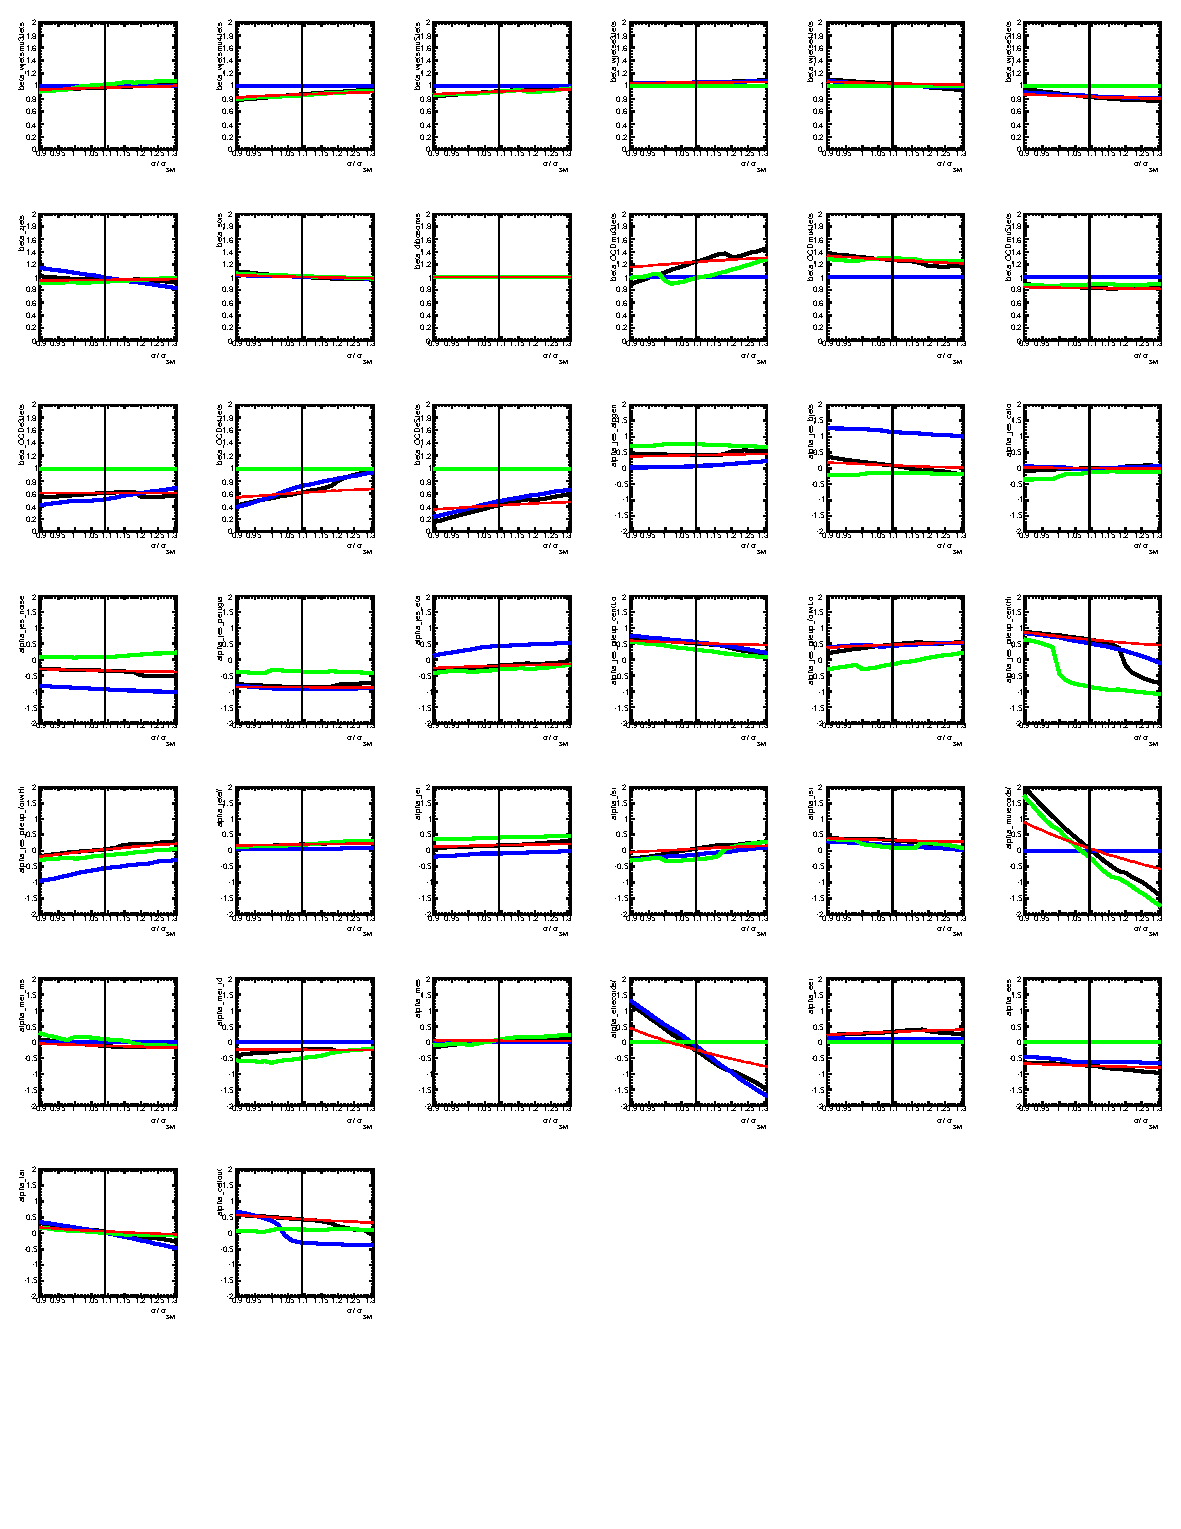
\includegraphics[width=\textwidth]{figures/comb/LJetsProfilePlots}
    \caption{The conditional maximum likelihood estimates $\hat{\hat{\alpha}}_j$ vs. $\sigma/\sigma_{\rm SM}$ for the single lepton analyses.  The results from the full likelihood of the individual channels $e+\textrm{jets}, \mu+\textrm{jets}$ are shown in blue and green, respectively, and the combined result is shown in black.  The red curve shows the approximation of the combined likelihood function with a multivariate Gaussian.  The vertical black line indicates the best fit signal cross-section, where the Gaussian approximation and the full combined likelihood should (and do) meet.  The scale of the $\alpha$ parameters is such that $\pm 1$ indicates $\pm 1\sigma$ uncertainty in the source of the systematic.}
    \label{fig:ljets_profile}
  \end{center}
\end{figure}





\subsection{Likelihood function for the Dilepton Analysis}
\label{sec:dilep}

The likelihood function for each of the dilepton channels consists of a single Poisson term for the number of observed events with $\ge2$ jets and several Gaussian constraint terms for the nuisance parameters $\vec{\alpha}$.   
These nuisance parameters are defined such that the nominal value of a systematic uncertainty corresponds to $\alpha_j = 0$ and a one standard deviation shift corresponds to $\alpha_j = \pm 1$.
These parameters are therefore constrained by Gaussian terms with means of 0 and standard deviations of 1.
Similarly, the parameter corresponding to the integrated luminosity, $\lum$, is constrained by a Gaussian term whose mean is the nominal value of the integrated luminosity, $\lum_{0}$, and whose standard deviation, $\sigma_{\lum}$, is equal to the uncertainty on the integrated luminosity.
The combined likelihood is given by the product of the Poisson terms and the Gaussian constraint terms

\begin{equation}\label{Eq:dileplikelihood}
  L_{ll}(\sigma_{\ttbar}, \lum, \vec{\alpha}) = \text{Gaus}(\lum_0 | \lum, \sigma_\lum)\, \prod_{i\in \{ ee,\mu\mu,e\mu\} }  \text{Pois}(N^{\text{obs}}_i \,|\, N^{\text{exp}}_{i, \text{tot}}(\vec{\alpha})\,) \,  \prod_{j\in \text{syst}} \text{Gaus}( 0 \,|\, \alpha_{j}, 1) \,,
\end{equation}
%where Pois is the Poisson distribution, Gaus is the Gaussian distribution, and the constraint terms on common systematic uncertainties are only included once.  
where constraint terms on common systematic uncertainties are only included once.  
%The Gaussian terms that constraint the parameters describing the effect of systematic uncertainties, $alpha_j$, are defined such that the measured value of a systematic corresponds to $alpha_j = 0$  their measured value in data i
The variation in the expected number of events from the signal and each background process is estimated from dedicated studies of each of the systematic effects.  
The total number of expected events, $N^{\text{exp}}_{i,\text{tot}}(\alpha_j)$, is then parametrized via piece-wise linear interpolation in the nuisance parameters $\alpha_j$ associated with each source of systematic uncertainty using the RooFit/RooStats software package~\cite{Verkerke:2003ir,Moneta:2010pm}.

%\begin{equation}\label{Eq:alphaInterpolation}
%N^{\text{exp}}_{i, \text{tot}}(\vec{\alpha}) = \sum_{\text{background}} N^{\text{exp}}_{i} (1 + \sum_{j} \alpha_{j} ( \mathbbm{1}_{ \alpha_{j} > 0} \, \Delta N^{+}_{j} - \mathbbm{1}_{ \alpha_{j} < 0} \, \Delta N^{-}_{j}   ) ) \, ,
%\end{equation}
%where $\mathbbm{1}$ is the indicator function whose value is 1 or 0 if its argument is true or false, respectively, and $\Delta N^{+}_{j}$ and $\Delta N^{-}_{j}$ are the differences in the expected number of events due to an updward or downward fluctuation of one standard deviation of the $j^{th}$ nuisance parameter. 

\begin{eqnarray}\label{Eq:alphaInterpolation}
N^{\text{exp}}_{i, \text{tot}}(\vec{\alpha}) &=& \sum_{\text{background}} N^{\text{exp}}_{i} (1 + \sum_{j} \alpha_{j} \, \Delta N_j  ) \, \\ 
\Delta N_j &=& \begin{cases} \Delta N^{+}_{j}, & \mbox{if } \alpha_{j} > 0  \\ \Delta N^{-}_{j}, & \mbox{if } \alpha_{j} < 0 \end{cases} , 
\end{eqnarray} 
where $\Delta N^{+}_{j}$ and $\Delta N^{-}_{j}$ are the differences in the expected number of events due to an upward or downward fluctuation of one standard deviation of the $j^{th}$ nuisance parameter. 

The dilepton likelihood function contains 65 parameters, including the parameter of interest, $\sigma_{\ttbar}$, the integrated luminosity, $\lum$, and 63 other nuisance parameters.
The profile likelihood ratios for the individual channels as well as the dilepton combination are shown in Figure~\ref{fig:dilep_profiles}.  
The dominant systematic uncertainties for the dilepton analysis are lepton identification efficiencies, fake lepton rates, modeling of the signal, and jet energy scale, which is modeled identically in the single-lepton and dilepton channels.
%To match the single-lepton analysis, the effect of the jet energy scale uncertainty is parameterized by several components, each of which is considered independent.
More information on the measurement using dilepton final states can be found in reference \cite{DILEPTON_PAPER}.

\begin{figure}[htbp]
  \begin{center}
    \subfigure[$ee$]{       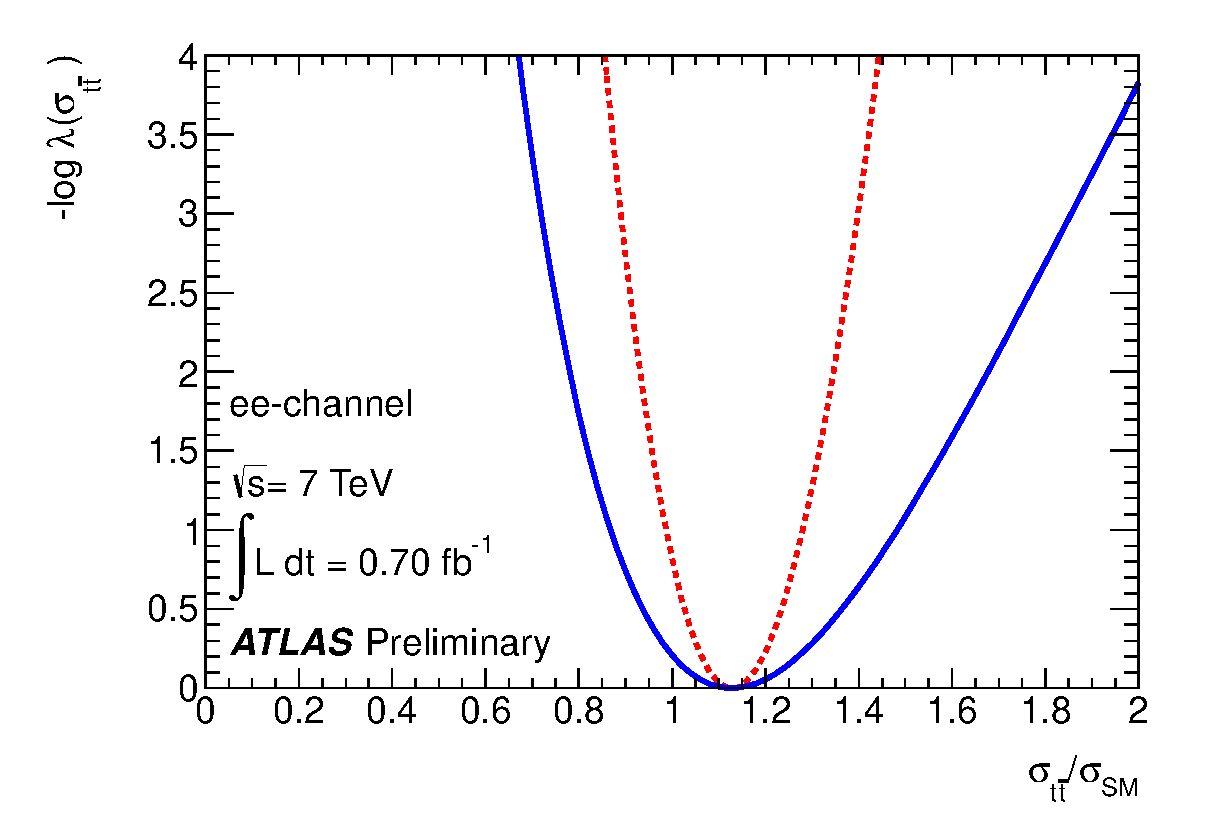
\includegraphics[width=.40\textwidth]{figures/comb/top_dilepton_ee_forComb_profileLR} }
     \subfigure[$\mu \mu$]{ 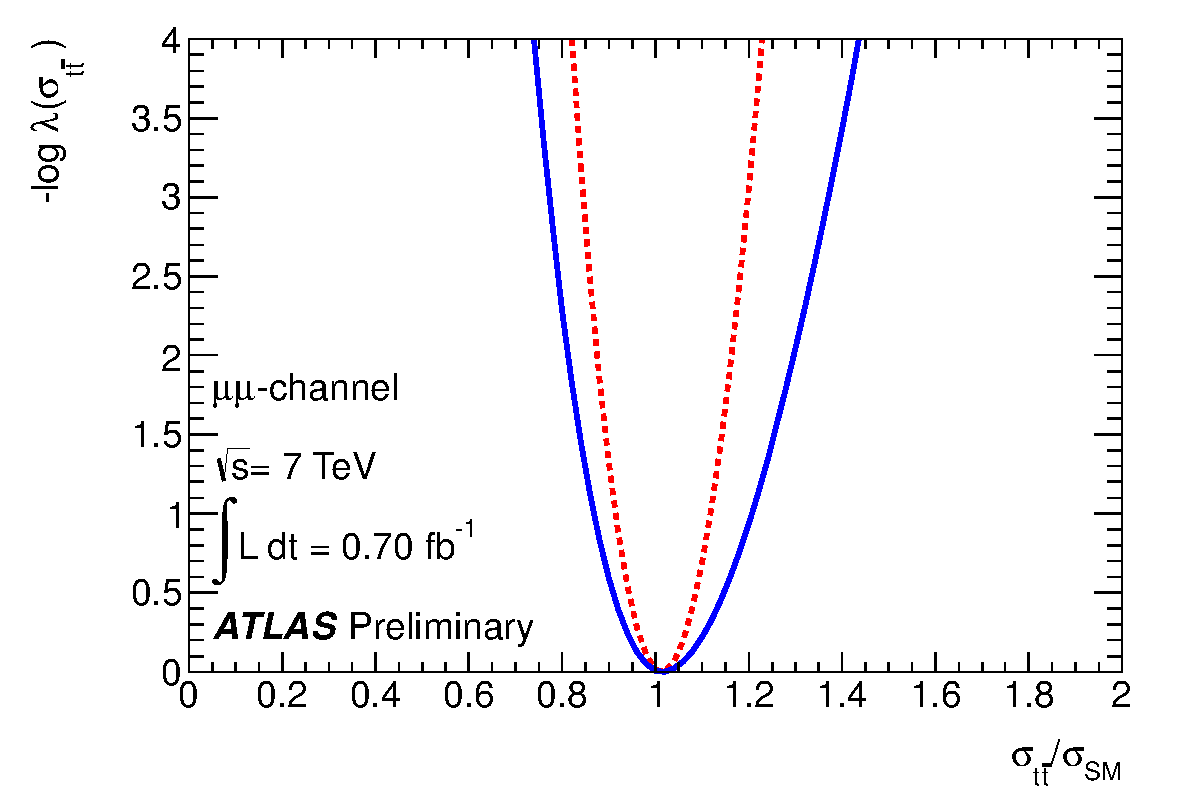
\includegraphics[width=.40\textwidth]{figures/comb/top_dilepton_mm_forComb_profileLR} }\\
     \subfigure[$e \mu$]{   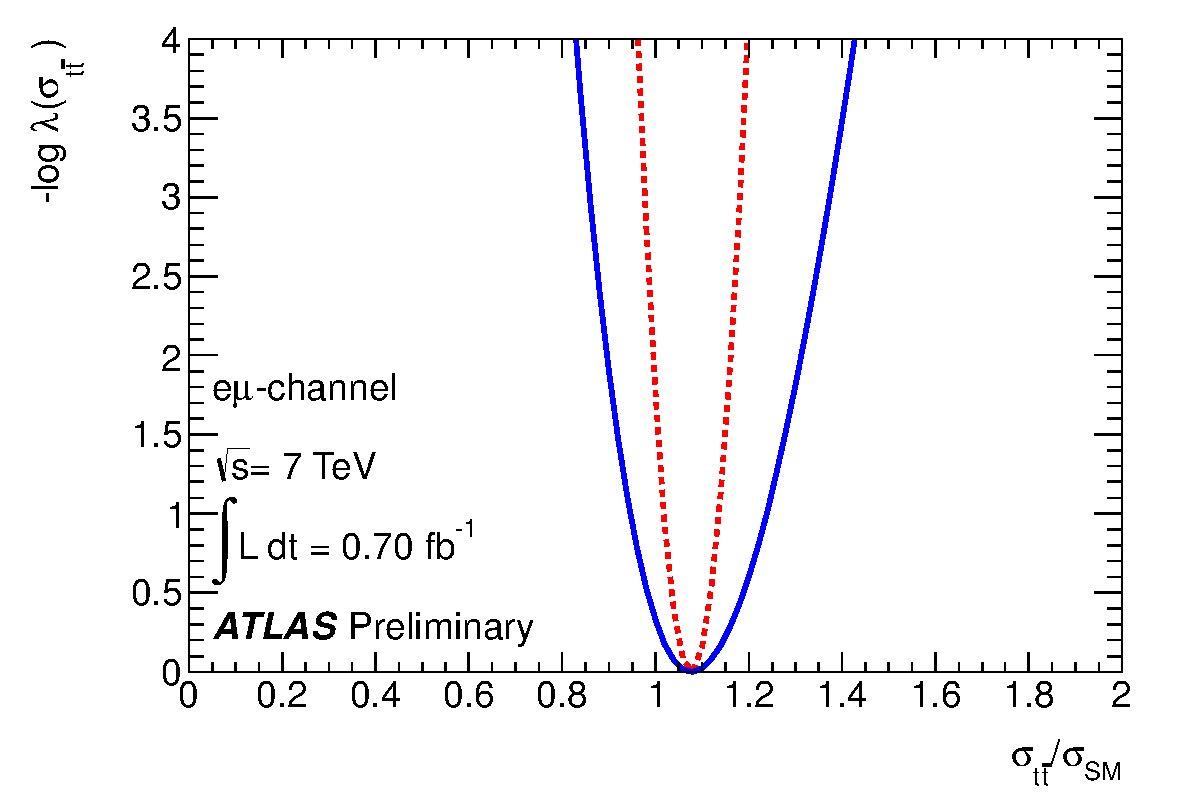
\includegraphics[width=.40\textwidth]{figures/comb/top_dilepton_em_forComb_profileLR} }
     \subfigure[Combined]{  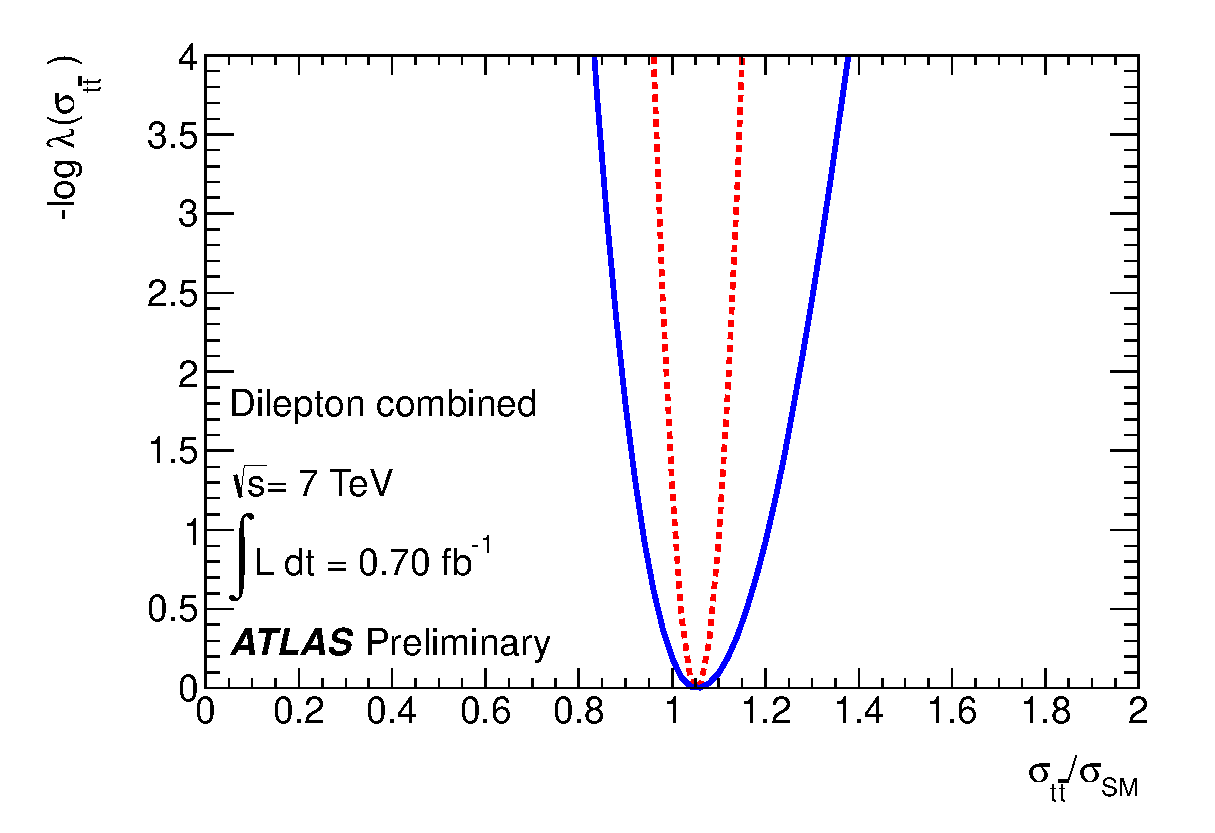
\includegraphics[width=.40\textwidth]{figures/comb/top_dilepton_combined_forComb_profileLR} }\\
    \caption{Graphs of $-\log\lambda(\sigma_{\ttbar})$ vs. $\sigma_{\ttbar}/\sigma_{\rm SM}$ with (blue, solid) and without (red, dashed) systematic uncertainties for the individual channels $ee$ (a), $\mu\mu$ (b), and $e\mu$ (c), and the three-channel combined fit (d).}
    \label{fig:dilep_profiles}
  \end{center}
\end{figure}

% INT ONLY
 \begin{figure}[htbp]
   \begin{center}
     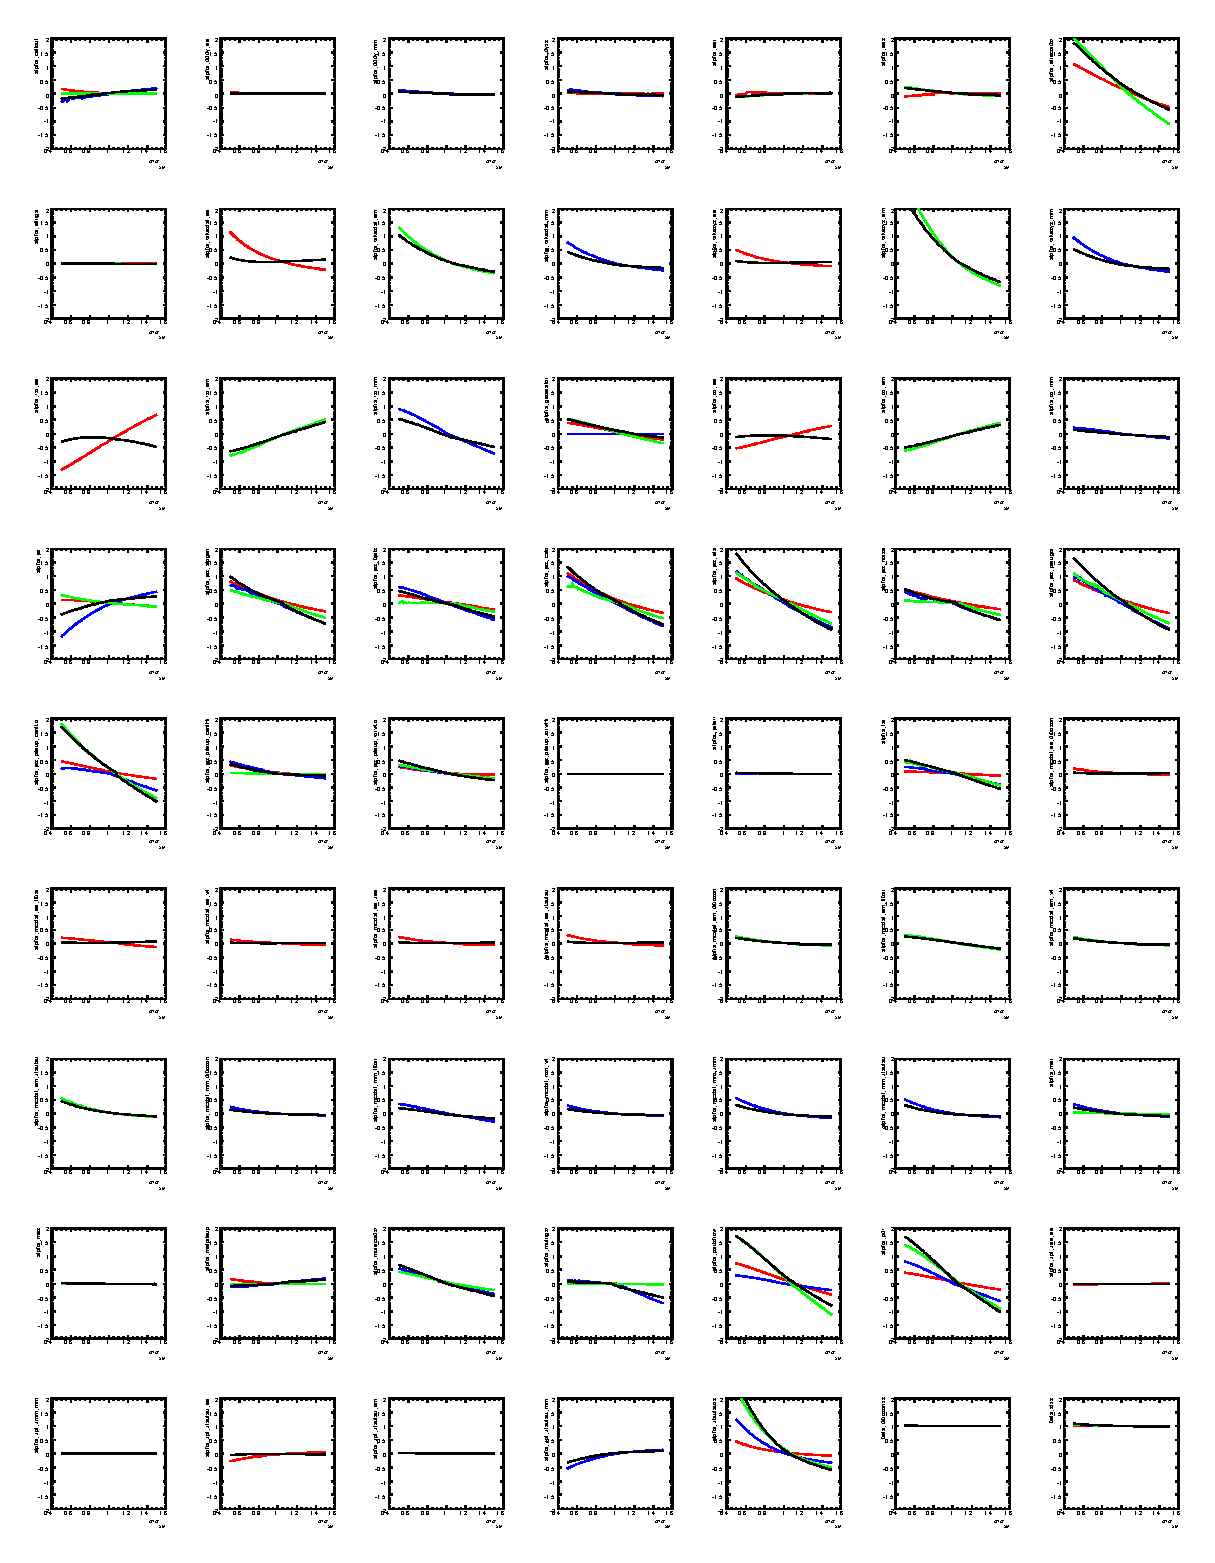
\includegraphics[width=\textwidth]{figures/comb/DilepProfilePlots}
    \caption{The conditional maximum likelihood estimates $\hat{\hat{\alpha}}_j$ vs. $\sigma/\sigma_{\rm SM}$ for the dilepton analyses.  The individual channels $ee, \mu\mu, e\mu$ are shown in red, blue, and green, respectively, and the combined result is shown in black.  The scale of the $\alpha$ parameters is such that $\pm 1$ indicates $\pm 1\sigma$ uncertainty in the source of the systematic.}
     \label{fig:dilepton_profile}
   \end{center}
 \end{figure}


\subsection{Likelihood function for the All Hadronic Analysis}
\label{sec:allhad}

The top quark cross-section is measured in the all-hadronic channel by performing a binned likelihood fit of signal and background templates to data.
The observable described by these templates is based on the reconstructed top-quark mass per event:
% of a $\chi^2$ of the reconstructed top-quark mass per event as a   discriminant''
% the minimum $\chi^2$d of the reconstructed top-quark mass:
%  kinematic fit assuming the $\ttbar$ event hypothesis
% $\chi^2$ distribution of the reconstructed top-quark mass to data

\begin{equation}\label{Eq:chisquare}
  \chi^2 =  \frac{ \left(m_{j_1, j_2} - m_{W}\right)^2}{\sigma_W^2} + \frac{ \left(m_{j_1, j_2, b_1} - m_{t}\right)^2}{\sigma_t^2} + \frac{ \left(m_{j_3, j_4} - m_{W}\right)^2}{\sigma_W^2} + \frac{ \left(m_{j_3, j_4, b_2} - m_{t}\right)^2}{\sigma_t^2},
  \end{equation}
where the particular jet combination used per event is the one that minimizes this sum~\cite{ATLAS-CONF-2011-140}.
% where the choice of jet labeling per event is the one that minimizes this $\chi^2$d.
% where the set of jets labeling that minimizes this $\chi^2$d per event is chosen.
% where the choice of jets per event is that which minimize this $\chi^2$d.
% where the combination of reconstructed objects that minimize this $\chi^2$ are used per event~\cite{allhad}.

The likelihood function for the all-hadronic channel consists of a product of Poisson terms, 
one for each of the 15 bins in the distribution of the $\chi^2$ value defined by equation~\ref{Eq:chisquare} above. 
The mean value for each bin is the sum of the signal and background templates, including the parametrized effects of systematic uncertainties.
%one for each of the 15 bins, describing the height of the $\chi^2$ distribution.
%The mean height for each bin is the sum of the signal and background templates, including the parametrized effects of systematic uncertainties.
%The signal template is generated using Monte Carlo simulation, and the background template, 
The signal template is generated using Monte Carlo simulation and the background template, which models the $\chi^2$ distribution in QCD multijet events, is extracted using a data-driven technique.
%These template distributions are each scaled by the luminosity, which is Gaussian constrained in the likelihood fit.
In total, the all-hadronic likelihood contains 22 parameters, including $\sigma_{\ttbar}$, the integrated luminosity, and 20 other nuisance parameters.
%The likelihood function used in this note was built using the RooFit/RooStats software package [9, 10]

The size of the systematic uncertainties in the all-hadronic channel are measured by fitting alternative templates of signal and background, 
each representing the plus or minus one standard deviation shift of an individual source of systematic uncertainty.
In the likelihood used for the combination, each source of systematic uncertainty enters as an overall scaling of the signal or background normalization,
the size of which is based on the measured uncertainties in the all-hadronic channel.
%These scalings are constrained by Gaussian terms such that a one standard deviation shift in the underlying parameter has an effect on the signal or background normalization equal to the measured size of each systematic.
The likelihood for the all-hadronic channel is given by

%\begin{equation}\label{Eq:dileplikelihood}
%  L_{had}(\sigma_{\ttbar}, \lum, \alpha_{j}) = \text{Pois}(N^{obs} \,|\, s(\alpha_j) + b(\alpha_j)) \prod_{i\in bins} \text{Pois}(n_{i} \,|\, s(\alpha_j) f_{i}^{s} \,+\, b(\alpha_j) f_{i}^{b})  \prod_{j\in \text{syst}} \text{Gaus}( 0 \,|\, \alpha_{j}, 1) \, \text{Gaus}(\lum_0 | \lum, \sigma_\lum)\,
%\end{equation}
\begin{equation}\label{Eq:dileplikelihood}
  L_{\text{had}}(\sigma_{\ttbar}, \lum, \vec{\alpha }) = \text{Gaus}(\lum_0 | \lum, \sigma_\lum)\, \prod_{i\in \text{bins}} \text{Pois}(n_{i} \,|\, s_{i}(\vec{\alpha}) \,+\, b_{i}(\vec{\alpha}))  \prod_{j\in \text{syst}} \text{Gaus}( 0 \,|\, \alpha_{j}, 1) \,  ,
\end{equation}
where $s_{i}(\vec{\alpha})$ and $b_{i}(\vec{\alpha})$ are the expected number of events from signal and background in the $i^{th}$ bin and $n_{i}$ is the observed number of events in the same bin. 

The largest sources of systematic uncertainty in the all-hadronic model are the jet energy scale, the $b-$tagging efficiency, and modeling of initial-state and final-state radiation.
Other significant sources of uncertainty include the jet energy resolution, the efficiency of the multijet trigger, and modeling of the multijet background.
Further details on cross-section measurement using all-hadronic final states can be found in reference~\cite{ATLAS-CONF-2011-140}.
The likelihood function for the all-hadronic channel is shown in Figure ~\ref{fig:allhad_likelihood}.

\begin{figure}[htbp]
  \begin{center}
    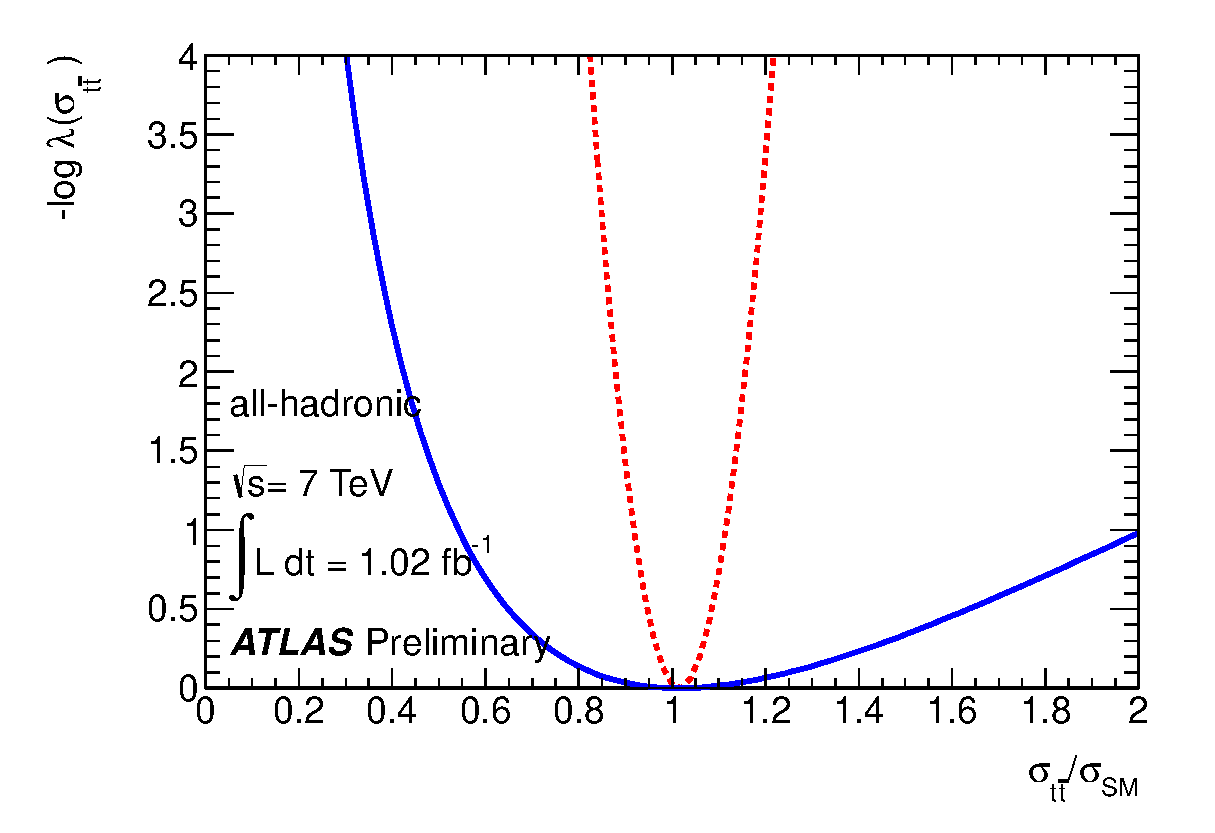
\includegraphics[width=.40\textwidth]{figures/comb/allhadronic_likelihood_curve}
  \caption{Graph of $-\log\lambda(\sigma_{\ttbar})$ vs. $\sigma_{\ttbar}/\sigma_{\rm SM}$ with (blue, solid) and without (red, dashed) systematic uncertainties for the all-hadronic channel.}
  \label{fig:allhad_likelihood}
  \end{center}
\end{figure}



\subsection{The Combined Likelihood}
\label{sec:comb}

The component analyses share several common sources of systematic uncertainty:
\begin{itemize}
\item electron and muon identification efficiencies,
\item electron energy scale and resolution,
\item muon momentum scale and resolution,
\item Monte Carlo generator, modeling of initial-state and final-state radiation,
\item jet energy resolution, jet energy scale, and jet efficiency,
\item calculation of missing transverse energy,
\item sporadic hardware failures which are not modeled in simulation,
\item background contributions from diboson and single top-quark events,
\item parton distribution functions and parton shower modeling,
\item integrated luminosity.
\end{itemize}

% The constraint terms $G(0|\alpha_j,1)$ associated with these common uncertainties cannot be double-counted.  

Sources of systematic uncertainty which are shared between channels are taken to be fully correlated.
The sources of uncertainty related to the modeling of the $\ttbar$ signal that are listed above are taken to be fully correlated because common Monte Carlo generators, parton distribution functions, and parton shower software were used across the single-lepton, dilepton, and all-hadronic analyses.
Experimental uncertainties, such as energy scales and identification efficiencies, that are listed above are correlated because they represent quantities that act coherently across channels and because they are modeled and evaluated using common techniques.
%  Systematic uncertainties that are correlated across channels
Constraint terms that are common to one or more of the single-lepton, dilepton or all-hadronic likelihoods appear only once in the full six-measurement likelihood.
%must be removed when forming the six-channel combination. 
% Because the likelihood function from the single-lepton analysis is approximated by a single multivariate Gaussian, constraint terms in the dilepton or all-hadronic likelihoods that are shared by the single-lepton likelihood must be removed when forming the six-channel combination. 
% Before combining, the dependence of the conditional maximum likelihood estimates, $\hat{\hat{\alpha}}_j$, as a function of $\sigma_{\ttbar}/\sigma_{\rm SM}$ were compared for the dilepton and single-lepton channels.  
% Those studies did not indicate any unexpected tension in the shared nuisance parameters that would indicate incompatible results.

%The final six-channel likelihood (equation \ref{Eq:combinedlikelihood}) is formed from a product of the approximate single-lepton likelihood, $L_{l+\rm jets}$, which includes the parameter of interest, $\sigma_{\ttbar}$, and 45 nuisance parameters (25 of which are shared with the dilepton channels, including a luminosity constraint), the Poisson terms corresponding to the cut-based analyses for the dileptons (which depend on the parameter of interest), the all-hadronic likelihood and Gaussian constraints for the remaining 28 nuisance parameters that only affect the dilepton channels.  
The final six-measurement likelihood (equation \ref{Eq:combinedlikelihood}) is formed from a product of the approximate single-lepton likelihood, the Poisson terms corresponding to the cut-based dilepton analyses, the template-based all-hadronic likelihood, and Gaussian constraint terms for the 43 nuisance parameters that are not constrained by the single-lepton likelihood.

%In total, there are 74 parameters in the six-channel combined fit.

\begin{eqnarray} \label{Eq:combinedlikelihood} \nonumber
  L_{\text{comb}}(\sigma_{\ttbar}, \lum, \vec{\alpha}) &=& L_{l+\rm jets}(\sigma_{\ttbar},\lum, \vec{\alpha})  \prod_{i\in \{ ee,\mu\mu,e\mu\} } 
   \text{Pois}(N^{\text{obs}}_i | N^{\text{exp}}_{i, \text{tot}}(\vec{\alpha}) ) \, \\ \nonumber 
   & & \times \,  \prod_{k\in \text{all-had bins}} \text{Pois}(n_{k} \,|\, s_{k}(\vec{\alpha}) \,+\, b_{k}(\vec{\alpha})) 
     \prod_{j \, \notin \, \text{l+jets sys} } \text{Gaus}( 0 | \alpha_{j}, 1) \, . \\
\end{eqnarray}


The full likelihood contains 89 parameters in all, 26 of which are shared between the dilepton and single-lepton likelihoods, and 12 of which are common to all three component likelihoods.

%\begin{equation}\label{Eq:combinedlikelihood}
%\begin{split}
%  L_{6\text{chan}}(\sigma_{\ttbar}, \lum, \alpha_{j}) = L_{l+\rm jets}(\sigma_{\ttbar},\lum, \alpha_{j})  \prod_{i\in \{ ee,\mu\mu,e\mu\} }  \text{Pois}(N^{\text{obs}}_i | N^{\text{exp}}_{i, \text{tot}}) \, \text{Pois}(N^{obs} \,|\, s(\alpha_j) + b(\alpha_j)) \prod_{i\in bins} \text{Pois}(n_{i} \,|\, s(\alpha_j) f_{i}^{s} \,+\, b(\alpha_j) f_{i}^{b}) \,  \\ 
%\prod_{j \notin {l+jets\, \text{sys}}} \text{Gaus}( 0 | \alpha_{j}, 1) \, \times \text{Gaus}(\lum_0 | \lum, \sigma_\lum)\,.
%\end{split}
%\end{equation}


% LocalWords:  dileptons


\subsection{Results}
\label{sec:results}
%\section{Results and conclusions}

The result of fitting the six-measurement combined model to the observed data is summarized in Table \ref{tab:results}, 
together with the input measurements.
The measured value of top quark pair production cross-section is
\begin{equation}
\hat\sigma_{\ttbar} =  177 \pm 3~\textrm{(stat.)} \sp {}^{+8}_{-7}~\textrm{(syst.)} \pm 7~\textrm{(lumi.)}~\textrm{pb} = 177 \sp {}^{+11}_{-10}~\textrm{pb}, \nonumber
\end{equation}
with the 68\% confidence interval inferred from the asymptotic properties of the profile likelihood ratio, which is shown in Figure~\ref{fig:fullcombined_likelihood_curve}.  
This interval includes the effect of all systematic and statistical uncertainties, including their correlated effects on the signal and backgrounds in the six channels.  

The statistical uncertainty is obtained by fixing all the nuisance parameters associated with underlying sources of systematic uncertainty to their best fit values.  
The systematic component of the total uncertainty is obtained by subtracting in quadrature the statistical contribution from the total uncertainty, keeping only the integrated luminosity fixed.
Finally, the uncertainty attributed to the integrated luminosity is obtained by subtracting in quadrature the combined systematic and statistical uncertainties from the total uncertainty.
%, ensuring that the quadratic sum of all three components is consistent with the uncertainty from all contributions.
The dominant systematic uncertainties in the six-measurement combination are listed in Table~\ref{tab:importantSystematics}. 
%, which include uncertainties from the signal event generator, lepton identification, the parton distribution function, the jet energy scale, and parton shower modeling, 
The systematic uncertainty attributed to a particular parameter is estimated by subtracting in quadrature the uncertainty obtained
while keeping that parameter fixed from the total uncertainty, keeping the integrated luminosity fixed throughout.
In total, 26 of the 88 nuisance parameters representing sources of systematic uncertainty are shared between one or more analysis and are treated as fully correlated.
%While 54 of the 78 uncertainties are in fact uncorrelated between the single-lepton and dilepton models, the remaining 24 systematic uncertainties are properly treated as correlated. 
%Several of these correlated terms can be effectively constrained from data using the profile likelihood technique, and the magnitude of these errors in the combination is smaller than that in the individual channels as more data is available in the combination to constrain them.

The combined cross-section and its statistical uncertainty are in good agreement with a simple approximate calculation in which $\sigma_{\ttbar}$ is estimated by a weighted average of the dilepton, single-lepton, and all-hadronic results.
% based on the inverse estimated by a weighted sum of the uncertainties of the dilepton and single-lepton results. 
The total systematic uncertainty measured in the full combination is only slightly larger than one would expect assuming fully uncorrelated uncertainties. 

Because the all-hadronic measurement has the largest total uncertainties of the component analyes, an auxiliary combination was performed using only the single-lepton and dilepton channels.
The fitted cross-section and its errors were found to agree, within rounding, with the values obtained in the nominal three-channel fit.
The size of individual systematic uncertainties in that fit varied only minimially from those obtained in the nominal fit.

The fitted values, uncertainties, and correlations to $\sigma_{ \ttbar }$ for all parameters that are shared by two or more analysis are shown in Table~\ref{tab:commonFittedParams}.
The uncertainties and correlations were measured using Minuit's HESSE algorithm.
With the exception of ``SigXsecOverSM'', ``dibosonxs'', ``stxs'', and ``Lumi'', which have nominal means of 1.0, all parameters nominally have a mean value of 0.0 and a nominal uncertainty of 1.0.

% INT ONLY

\begin{table}[htbp]

  \begin{center}  
    \tiny
    \begin{tabular}{|r|ccc|ccc|ccc|ccc|} 
      \hline
      Common & \multicolumn{3}{|c|}{Dilepton}  & \multicolumn{3}{|c|}{Single-Lepton} & \multicolumn{3}{|c|}{All-Hadronic} & \multicolumn{3}{|c|}{Combined} \\
      \hline
      Uncertainty source & Value & Error & Corr. & Value & Error & Corr. & Value & Error & Corr. & Value & Error & Corr. \\
      \hline
       % Dilep
 %  \begin{table}[htbp]
 %       \begin{center}
 %         \small
 %       \begin{tabular}{|r|ccc|ccc|ccc|} \hline
 %         Common & \multicolumn{3}{|c|}{Dilepton}  & \multicolumn{3}{|c|}{Single Lepton} & \multicolumn{3}{|c|}{Combined} \\
 %         \hline
 %        Uncertainty source & Value & Error & Correlation & Value & Error & Correlation & Value & Error & Correlation \\
 %        \hline
Lumi  & 1.00 & 0.04 & -0.51  & 1.00 & 0.04 & -0.56  & 1.00 & 0.04 & -0.08  & 1.00 & 0.04 & -0.65  \\
SigXsecOverSM  & 1.05 & 0.09 & 1.00  & 1.09 & 0.07 & 1.00  & 1.01 & 0.45 & 1.00  & 1.08 & 0.07 & 1.00  \\
cellout  & 0.05 & 0.99 & 0.04  & 0.45 & 0.46 & -0.09 & XXX & XXX & XXX & 0.44 & 0.46 & -0.08  \\
eer  & 0.00 & 1.13 & 0.01  & 0.32 & 0.76 & 0.04 & XXX & XXX & XXX & 0.31 & 0.76 & 0.02  \\
ees  & 0.02 & 1.11 & -0.02  & -0.74 & 0.59 & -0.04 & XXX & XXX & XXX & -0.74 & 0.59 & -0.03  \\
elrecoidsf  & 0.23 & 0.93 & -0.21  & -0.23 & 0.92 & -0.22 & XXX & XXX & XXX & 0.03 & 0.85 & -0.25  \\
fsr  & -0.12 & 0.54 & -0.05  & 0.07 & 0.21 & 0.17  & -0.00 & 0.99 & -0.36  & 0.04 & 0.20 & 0.09  \\
generator  & 0.09 & 0.98 & -0.05  & -0.00 & 0.99 & -0.46  & -0.00 & 0.99 & -0.12  & 0.10 & 0.92 & -0.36  \\
isr  & -0.05 & 0.57 & 0.02  & 0.34 & 0.20 & -0.10  & -0.00 & 0.99 & -0.36  & 0.32 & 0.20 & -0.07  \\
jer  & 0.14 & 0.97 & 0.06  & 0.17 & 0.95 & 0.02  & -0.00 & 0.99 & -0.29  & 0.24 & 0.88 & 0.07  \\
jes\_alpgen  & 0.04 & 1.11 & -0.08  & 0.42 & 0.41 & 0.03 & XXX & XXX & XXX & 0.44 & 0.41 & 0.04  \\
jes\_bjets  & -0.02 & 0.87 & -0.08  & 0.10 & 0.68 & -0.05  & -0.00 & 0.99 & -0.05  & 0.05 & 0.56 & -0.05  \\
jes\_calo  & 0.04 & 1.07 & -0.13  & 0.01 & 0.43 & -0.01  & -0.00 & 0.99 & -0.13  & -0.02 & 0.42 & -0.04  \\
jes\_eta  & 0.01 & 1.21 & -0.23  & -0.19 & 0.21 & 0.10  & -0.00 & 0.99 & -0.13  & -0.19 & 0.21 & 0.06  \\
jes\_noise  & 0.03 & 1.32 & -0.04  & -0.35 & 0.40 & -0.04  & -0.00 & 0.99 & -0.07  & -0.35 & 0.40 & -0.04  \\
jes\_perugia  & 0.03 & 1.18 & -0.22  & -0.86 & 0.17 & -0.01  & -0.00 & 0.99 & -0.15  & -0.86 & 0.17 & -0.00  \\
jes\_pileup\_centHi  & -0.01 & 0.91 & -0.02  & 0.64 & 0.47 & -0.15 & XXX & XXX & XXX & 0.62 & 0.46 & -0.13  \\
jes\_pileup\_centLo  & 0.09 & 0.98 & -0.19  & 0.52 & 0.17 & -0.14 & XXX & XXX & XXX & 0.52 & 0.17 & -0.11  \\
jes\_pileup\_forwHi  & -0.00 & 0.99 & -0.00  & 0.04 & 0.91 & 0.08 & XXX & XXX & XXX & 0.05 & 0.90 & 0.06  \\
jes\_pileup\_forwLo  & -0.01 & 1.13 & -0.06  & 0.47 & 0.26 & 0.11 & XXX & XXX & XXX & 0.46 & 0.26 & 0.07  \\
jeteff  & 0.00 & 0.99 & -0.00  & 0.20 & 0.14 & 0.09  & -0.00 & 0.99 & -0.00  & 0.20 & 0.14 & 0.07  \\
lar  & -0.02 & 1.12 & -0.12  & 0.06 & 0.51 & -0.07  & -0.00 & 0.99 & -0.01  & 0.06 & 0.51 & -0.07  \\
mes  & -0.00 & 0.99 & -0.01  & 0.04 & 1.07 & -0.00 & XXX & XXX & XXX & 0.04 & 1.07 & -0.01  \\
murecoidsf  & -0.05 & 0.99 & -0.11  & 0.09 & 0.81 & -0.31 & XXX & XXX & XXX & 0.13 & 0.81 & -0.29  \\
partshow  & 0.15 & 0.96 & -0.25  & -0.00 & 0.99 & -0.08 & XXX & XXX & XXX & 0.21 & 0.91 & -0.16  \\
pdf  & 0.01 & 0.99 & -0.27  & -0.00 & 0.99 & -0.15  & -0.00 & 0.99 & -0.19  & -0.02 & 0.96 & -0.26  \\
dibosonxs  & 1.00 & 0.07 & -0.02  & 1.00 & 0.06 & -0.01 & XXX & XXX & XXX & 1.00 & 0.06 & -0.01  \\
stxs  & 1.00 & 0.12 & -0.06  & 1.00 & 0.11 & -0.08 & XXX & XXX & XXX & 1.00 & 0.11 & -0.09  \\
 %         \hline
 %   \end{tabular}
 %  \end{center}
 %  \caption{\label{tab:commonSystematics}
 %    Sources of systematic uncertainty that are common to the single lepton and dilepton channels.  
 %   Shown for each systematic uncertainty is the fitted value, error on the fitted value, and the correlation coeficient
 %   between the parameter and $\sigma_{	tbar}$.
 %   Results are shown for the dilepton model, the single lepton model, and the combined six-channel model.
 % }
 % \end{table}

      \hline
    \end{tabular}
  \end{center}
  \caption{ \label{tab:commonFittedParams} Sources of systematic uncertainty that are common to the single lepton and dilepton channels.  Shown for each systematic uncertainty is the fitted value, error on the fitted value, and the correlation coeficient between the parameter and $\sigma_{\ttbar}$.  Results are shown for the dilepton model, the single lepton model, the all-hadronic model, and the combined six-channel model. }
\end{table}

Because the all-hadronic measurement has the largest total uncertainties of the component analyes, an auxiliary combination was performed using only the single-lepton and dilepton channels.
The fitted cross-section and its errors were found to agree, within rounding, with the values obtained in the nominal three-channel fit.
The size of individual systematic uncertainties in that fit varied only minimially from those obtained in the nominal fit.

In the full fit, systematics that are common between analyses are described by a single parameter and therefore the systematic effects for those uncertainties across channels are fully correlated.
To test the self-consistency of extracted errors on the total fit and to better understand the effect of correlated systematics across channels, 
we ran several fits of our model comparing various treatments of the most important common systematic uncertainties.
These sources of uncertainty consisted of initial-state and final-state radiation, the jet energy scale, the Monte-Carlo generator, and the parton distribution function.
For each uncertainty, we first treated it as independent across the input models.  
We did this to test for any artificial overconstraining that may occur across likelihoods.
We then artificially shifted each source of uncertainty to their plus one, zero, and minus one standard deviation values and fixed them in a fit. 
The movement in the mean value of the cross section between these fits matches well the extracted errors described in table~\ref{tab:importantSystematics}.
The result of these fits are shown in Table~\ref{tab:SystematicDecorrelation}. 

\begin{table}[htbp]

  \begin{center}
    \begin{tabular}{|c|ccc|}
      \hline
      Fit Version & $\sigma_{\ttbar}$ (pb) & error up (pb) & error down (pb)  \\
      \hline
      \hline
      Standard Fit & 177.2 & 11.1 & -10.2\\
\hline 
Uncorrelated FSR & 177.7 & 11.1 & -10.3\\
Uncorrelated ISR & 177.2 & 11.1 & -10.2\\
ISR/FSR at +1 sigma & 179.4 & 10.8 & -10.3\\
ISR/FSR at 0 sigma & 178.6 & 11.0 & -10.3\\
ISR/FSR at -1 sigma & 177.7 & 11.0 & -10.3\\
\hline 
Uncorrelated JES & 176.9 & 11.6 & -10.6\\
JES at +1 sigma & 175.9 & 11.2 & -10.6\\
JES at 0 sigma & 176.4 & 11.5 & -10.5\\
JES at -1 sigma & 179.0 & 11.4 & -10.5\\
\hline 
Uncorrelated Generator & 177.7 & 11.1 & -10.2\\
Generator at +1 sigma & 173.9 & 10.0 & -9.5\\
Generator at 0 sigma & 177.8 & 10.5 & -9.6\\
Generator at -1 sigma & 182.2 & 10.7 & -9.9\\
\hline 
Uncorrelated Pdf & 177.4 & 11.0 & -10.1\\
Pdf at +1 sigma & 174.8 & 10.5 & -10.0\\
Pdf at 0 sigma & 177.4 & 10.9 & -9.9\\
Pdf at -1 sigma & 180.2 & 11.0 & -10.1\\

      \hline
    \end{tabular}
  \end{center}
  \caption{ \label{tab:SystematicDecorrelation} Table of the fitted value of $\sigma_{ \ttbar }$ and its asymmetric errors for various treatments of important systematic uncertainties: initial-state and final-state radiation, jet energy scale, Monte-Carlo generator, and the parton distribution function.   }
\end{table}




% Note, the dilepton numbers differ from those in the
% dilepton paper due to the use of separated jes.
\begin{table}[htdp]
  \begin{center}
    \begin{tabular}{|l|c|}\hline
      Channel & $\sigma_{\ttbar}$ (pb) \\ 
      \hline
      & \\
      Single-lepton combined & $179 \pm  4  \textrm{(stat.)} \pm 9           \textrm{(syst.)}  \pm 7 \textrm{(lumi.)}$ \\
      & \\
      \hline
      & \\
      $ee$      & $186 \pm 17  \textrm{(stat.)} \sp {}^{+31}_{-26} \textrm{(syst.)} \sp {}^{+9}_{-7} \textrm{(lumi.)}$ \\ 
      & \\
      $\mu\mu$  & $167 \pm 12 \textrm{(stat.)}  \sp {}^{+15}_{-11} \textrm{(syst.)} \sp {}^{+8}_{-7} \textrm{(lumi.)}$ \\ 
      & \\
      $e\mu$    & $177 \pm 7  \textrm{(stat.)}  \sp {}^{+15}_{-12} \textrm{(syst.)} \sp \pm 8        \textrm{(lumi.)}$ \\ 
      & \\
      % \hline
      % & \\
      Dilepton combined & $173 \pm 6  \textrm{(stat.)}  \sp {}^{+14}_{-11} \textrm{(syst.)} \sp {}^{+8}_{-7} \textrm{(lumi.)}$ \\
      & \\
      \hline
      & \\
      All-hadronic           & $167 \pm  18 \textrm{(stat.)} \pm 78           \textrm{(syst.)} \pm 6 \textrm{(lumi.)}$ \\
      & \\ 
      \hline 
      \hline
      & \\
      Combined   & $177 \pm  3 \textrm{(stat.)}  \sp {}^{+8}_{-7} \textrm{(syst.)} \pm 7 \textrm{(lumi.})$ \\
      & \\ 
      \hline
    \end{tabular}
  \end{center}
  \caption{\label{tab:results}
    %Measured values of $\sigma_{\ttbar}$ in each of the comsix individual analyses, the dilepton and single-lepton combinations, and the full six-channel combination.  
    Measured values of $\sigma_{\ttbar}$ obtained by the single-lepton measurement ($e+$jets and $\mu+$jets combined), the three component dilepton measurements ($ee$, $e \mu$ and $\mu \mu$) and well as the three-channel dilepton combination, the all-hadronic measurement, and the full combination of single-lepton, dilepton, and all-hadronic measurements.
  }

\end{table}



% Dilep
\begin{table}[htbp]
  \begin{center}
    \begin{tabular}{|l|c|} \hline
      Uncertainty source & Uncertainty (pb) \\
      \hline
      \hline
      Signal modeling uncertainties & \\
      \hline
      Event generator & +3.8 / $-$3.4 \\
      Parton shower modeling &  +2.0 / $-$1.9 \\
      Initial-state and final-state radiation & $\pm$ 1.2 \\ % +1.2 / $-$1.2 \\
      Parton distribution function & +2.9 / $-$2.7 \\
      \hline
      \hline
      Detector modeling & \\
      \hline
      Muon identification & +3.3 / $-$3.1 \\      
      Electron identification &  +2.9 / $-$2.7 \\
      Jet energy scale &  +2.4 / $-$2.3 \\
      Jet efficiency &  $\pm$ 0.8 \\ %+0.8 / $-$0.8 \\
      Missing transverse momentum & $\pm$ 0.9 \\% +0.9 / $-$0.9 \\
      \hline
      \hline
      Background from data & \\
      \hline
      Fake lepton estimate &  +1.4 / $-$1.3 \\
      Shape of single-lepton QCD template &  +0.6 / $-$0.5 \\
      \hline
      \hline
      Background from Monte Carlo & \\
      \hline
      Shape of single-lepton $W + \text{jets}$ template &  +0.7 / $-$0.6 \\
      \hline
      \hline
      All others & +2.6 / $-$2.5 \\
      \hline
    \end{tabular}
  \end{center}
  \caption{\label{tab:importantSystematics}
    Dominant sources of systematic uncertainty in the full combined likelihood 
    and their contribution to the error on the measured cross section.
  }
\end{table}



\begin{figure}[ht!]
  \begin{center}
    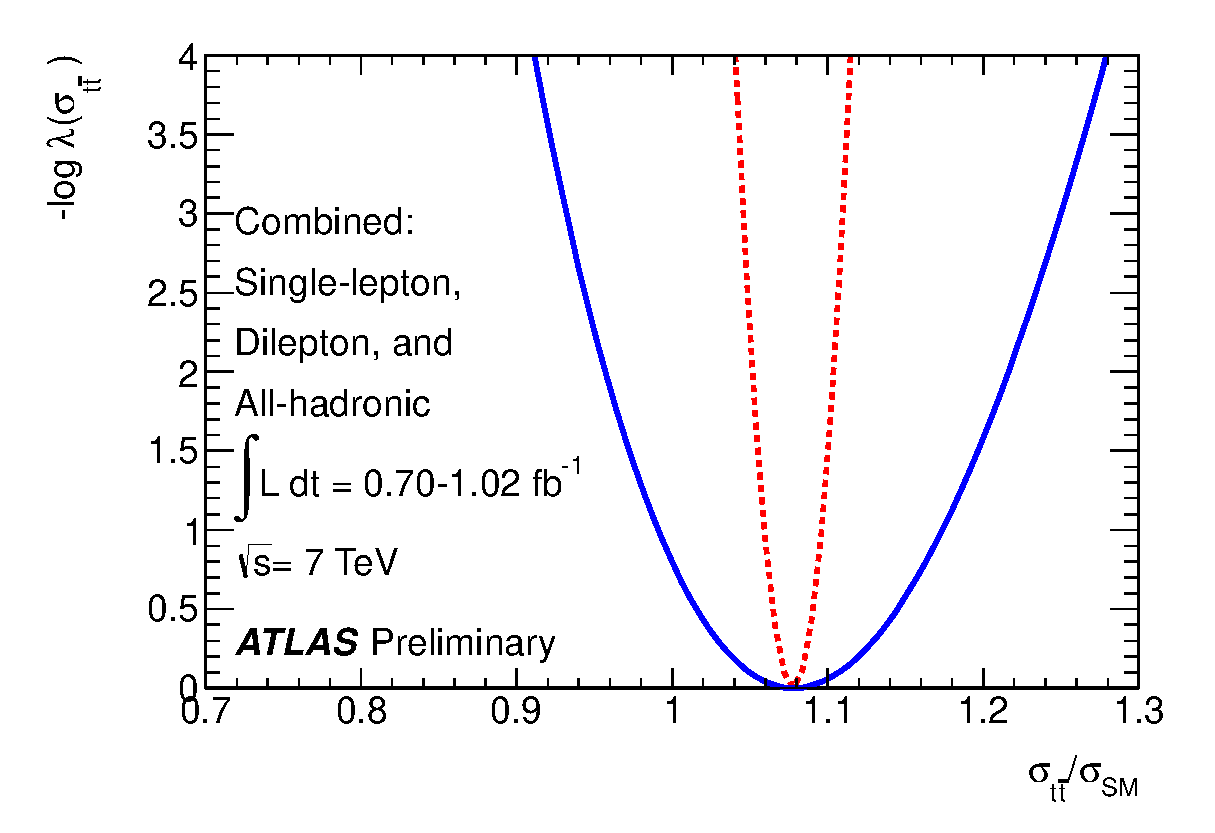
\includegraphics[width=.7\textwidth]{figures/comb/fullcombined_likelihood_curve}
    \caption{Graph of $-\log\lambda(\sigma_{\ttbar})$ vs. $\sigma_{\ttbar}/\sigma_{\rm SM}$ with (blue, solid) and without (red, dashed) systematic uncertainties for the six-channel combined fit.}
    \label{fig:fullcombined_likelihood_curve}
  \end{center}
\end{figure}



%This note presents a determination of the top quark pair production cross-section using a statistical combination of single-lepton, dilepton, and all-hadronic final states.
%The measured value, $\hat\sigma_{\ttbar} = 177 \pm 3~\textrm{(stat.)} \sp {}^{+8}_{-7}~\textrm{(syst.)} \pm 7~\textrm{(lumi.)}~\textrm{pb}$, is in good agreement with the Standard Model prediction.
Figure~\ref{fig:summary_summary} shows a summary of the cross-section measurements made by ATLAS that are combined in this note as well as the result obtained by this combination.
This measurement, which has a total uncertainty of 6\%, has a smaller relative uncertainty than recent Tevatron cross-section combinations, which measured $7.50 \pm 0.48~\textrm{pb}$ at $\sqrt{s}= 1.96\, \TeV$ for an uncertainty of 6.4\%~\cite{CDFCombination}.
Figure~\ref{fig:xsec_vs_roots} shows various cross-section measurements from Tevatron and ATLAS experiments overlaid on the theoretical predictions as a function of center-of-mass energy.

\begin{figure}[ht!]
  \begin{center}
    % 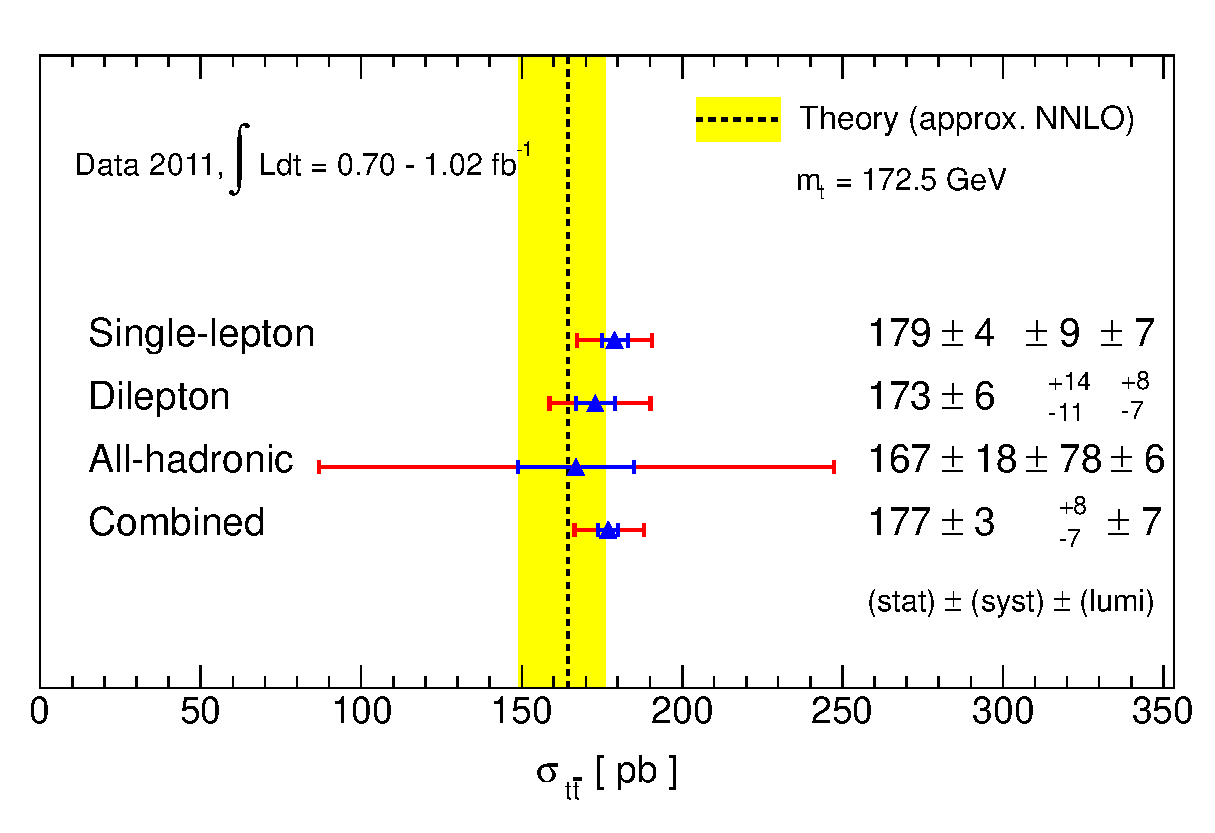
\includegraphics[width=.7\textwidth]{figures/comb/summary_summary.eps}
    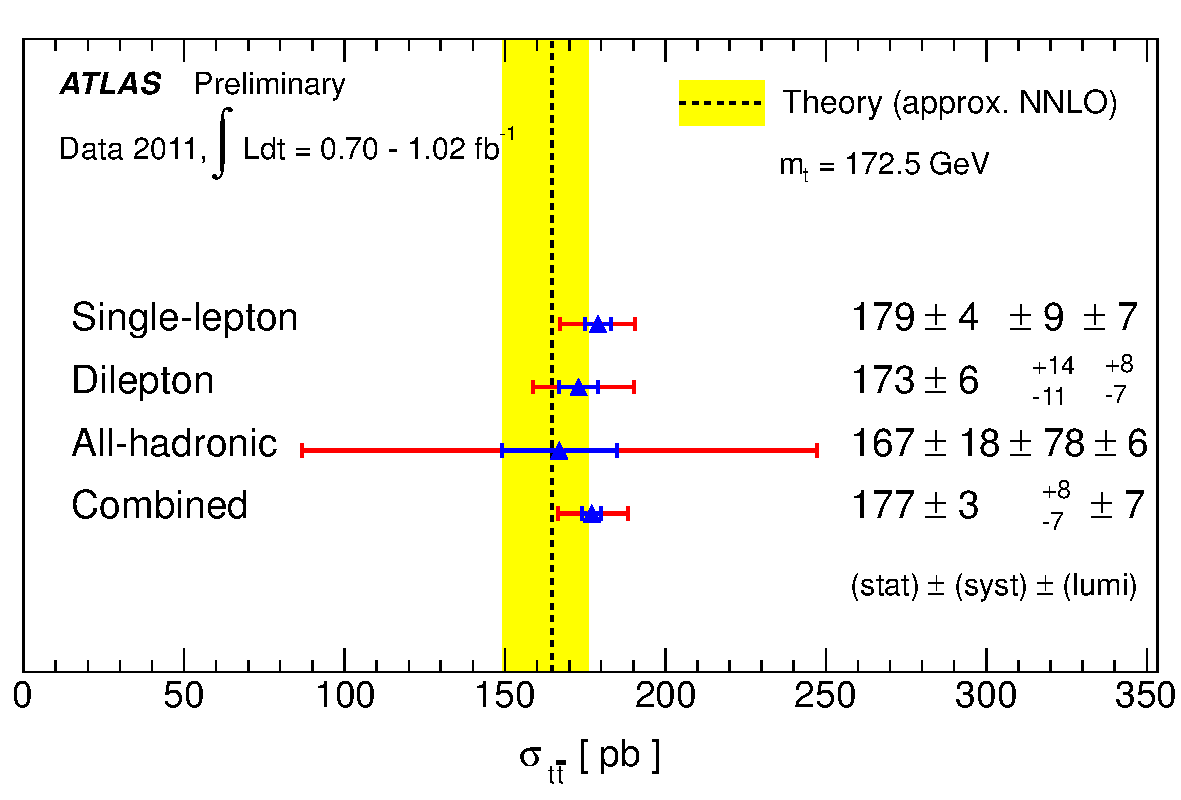
\includegraphics[width=.8\textwidth]{figures/comb/summary_summary_atlprelim}
    \caption{The measured value of $\sigma_{\ttbar}$ in the single-lepton channel, the dilepton channel, the all-hadronic channel, and the combination of these three measurements, including error bars for both statistical uncertainties only (blue) and including systematic uncertainties (red).  The approximate NNLO prediction with its uncertainty (yellow) is also shown.}
    \label{fig:summary_summary}
  \end{center}
\end{figure}


\begin{figure}[ht!]
  \begin{center}
    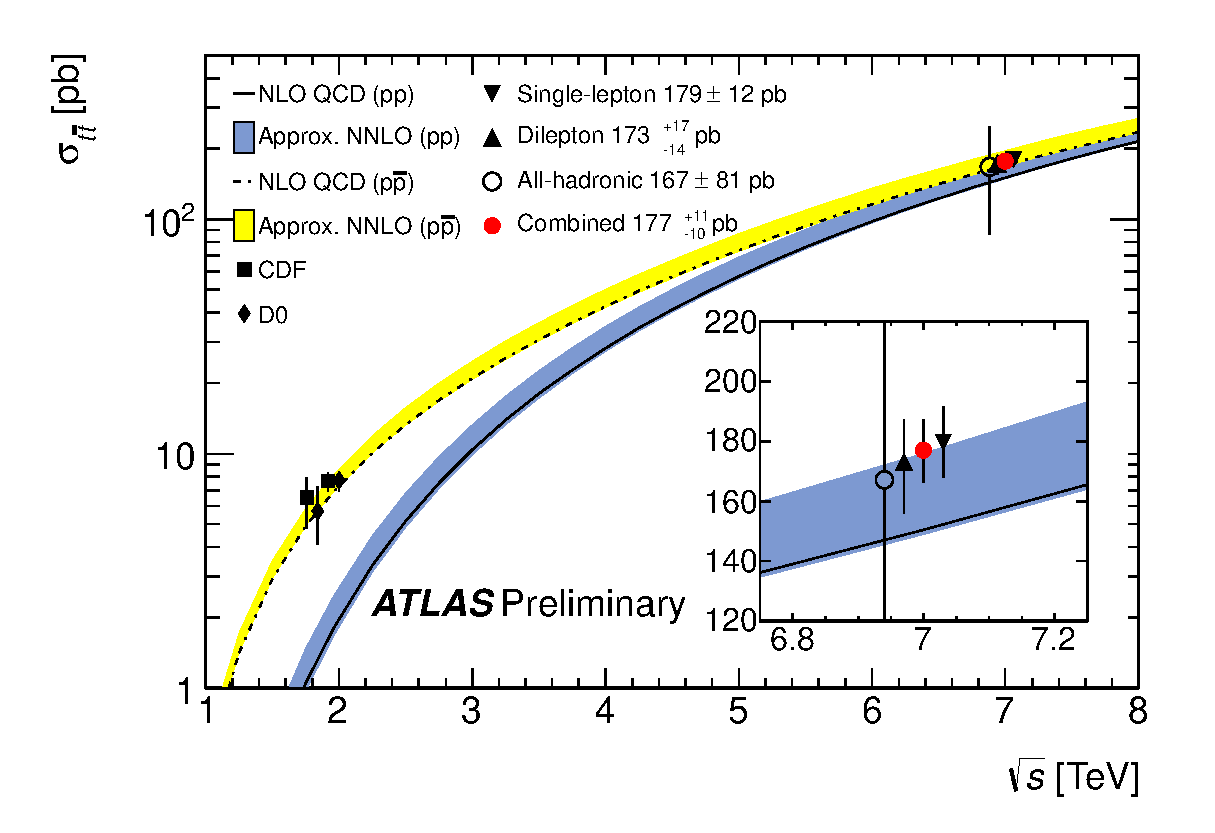
\includegraphics[width=.8\textwidth]{figures/comb/top_crosssection_rootS.eps}
    \caption{Dependence of $\sigma_{\ttbar}$ on $\sqrt{s}$ from theoretical predictions based on a top-quark mass of 172.5 GeV together with the dilepton, single-lepton, and all-hadronic measurements from ATLAS, as well as the combined measurement presented in this note.  Uncertainties on measurements are shown as vertical error bars and include statistical, systematic, and luminosity contributions.  Selected results obtained by Tevatron experiments are also shown~\cite{CDF1p8,CDF2p6,D01p8,D04p3}. Measurements made at the same center-of-mass energy are slightly offset for clarity. }
    \label{fig:xsec_vs_roots}
  \end{center}
\end{figure}


